\documentclass[sigconf]{acmart}

\usepackage{booktabs} % For formal tables
\usepackage{verbatim}
\usepackage{soul}
\usepackage{color,calc}
\PassOptionsToPackage{bookmarks=false}{hyperref}
\usepackage{listings}
\usepackage{tcolorbox}
\usepackage{comment}
\usepackage{xspace}
\usepackage{subcaption}
\usepackage{multirow}
\usepackage{tikz}
\usepackage{color, colortbl}
\usepackage{flushend}
\usepackage[skip=10pt]{caption}

%\usepackage[labelformat=simple]{subcaption}
\usepackage[disabled]{aplcomments}

%\usepackage[inline]{aplcomments}
\newcommenter{shan}{1.0,0.0,0.0}
\newcommenter{junwen}{0.0,1.0,0.0}
\newcommenter{utsav}{1.0, 0.5, 0.0}
\newcommenter{cong}{0.0,0.8,0.8}
\newcommenter{alvin}{0.0,1.0,1.0}
%\usepackage[disabled]{aplcomments}
%\renewcommand\footnotetextcopyrightpermission[1]{} 
\usepackage[justification=centering]{caption}
\usepackage{flushend}
\usepackage[labelformat=simple]{subcaption}
\newcommand{\seclabel}[1]{\label{s:#1}}
\newcommand{\lstlabel}[1]{\label{lst:#1}}
\newcommand{\figlabel}[1]{\label{f:#1}}
\settopmatter{printacmref=false}


\newcommand{\tabref}[1]{Table~\ref{table:#1}}
\newcommand{\figref}[1]{Figure~\ref{fig:#1}}
\newcommand{\secref}[1]{Section~\ref{sec:#1}}
\newcommand{\secrefs}[2]{Sections~\ref{sec:#1}-\ref{sec:#2}}
\newcommand{\ssecref}[1]{Sec.~\ref{sec:#1}}
\newcommand{\appref}[1]{Appendix~\ref{sec:#1}}
\newcommand{\algref}[1]{Algorithm~\ref{alg:#1}}
\newcommand{\listref}[1]{Listing~\ref{list:#1}}


\newcommand{\numissues}{114\xspace}
\newcommand{\numreportedissues}{56\xspace}
\newcommand{\numconfirmedissues}{49\xspace}
\newcommand{\numunconfirmedissues}{7\xspace}
\newcommand{\nummergedissues}{23\xspace}

\newcolumntype{L}[1]{>{\raggedright\arraybackslash}p{#1}}
\newcolumntype{R}[1]{>{\raggedleft\arraybackslash}p{#1}}

%\setcopyright{none}
\def\BibTeX{{\rm B\kern-.05em{\sc i\kern-.025em b}\kern-.08em
    T\kern-.1667em\lower.7ex\hbox{E}\kern-.125emX}}
    
\begin{abstract}
Database-backed web applications manipulate large amounts of persistent data, and such applications often contain constraints that restrict data length, data value, and other data properties. Such constraints are critical in ensuring the reliability
and usability of these applications.
%There are often constraints associated with data used in software, restricting data length, value, uniqueness, and other properties. These constraints are particularly crucial for the reliability, maintainability, and usability of database-backed web applications, where a huge amount of structured data is expected to persist in database and serve web users throughout software upgrade and database migration.
In this paper, we present a comprehensive study on where data constraints are expressed, what they are about, how often they evolve, and how their violations are handled. The results show that developers struggle with maintaining consistent data constraints and checking them across different components and versions of their web applications, leading to various problems.
%led to many real-world software reliability, maintainability, and usability problems. 
Guided by our study, we developed checking tools and API enhancements that can automatically detect such problems and improve the quality of such applications.

%problems in data-constraint specification and violation handling.

\end{abstract}
\begin{document}

\copyrightyear{2020} 
\acmYear{2020} 
\setcopyright{acmcopyright}
\acmConference[ICSE '20]{42nd International Conference on Software Engineering}{May 23--29, 2020}{Seoul, Republic of Korea}
\acmBooktitle{42nd International Conference on Software Engineering (ICSE '20), May 23--29, 2020, Seoul, Republic of Korea}
\acmPrice{15.00}
\acmDOI{10.1145/3377811.3380375}
\acmISBN{978-1-4503-7121-6/20/05}

\title{
Managing data constraints in database-backed web applications
% {\footnotesize}
%\thanks{http://hyperloop.cs.uchicago.edu/panorama}
}

 \author[J. Yang]{Junwen Yang}
\affiliation{
University of Chicago \country{USA} 
}
\email{junwen@uchicago.edu}
 \author[U. Sethi]{Utsav Sethi}
\affiliation{
 University of Chicago\country{USA} 
}
\email{usethi@uchicago.edu}
 \author[C. Yan]{Cong Yan}
\affiliation{University of Washington\country{USA} 
}
\email{congy@cs.washington.edu}

 \author[A. Cheung]{Alvin Cheung}
\affiliation{
  University of California, Berkeley\country{USA} 
}
\email{akcheung@cs.berkeley.edu}

 \author[S. Lu]{Shan Lu}
\affiliation{
  University of Chicago\country{USA} 
}
\email{shanlu@uchicago.edu}

\pagestyle{plain}

\maketitle

\section{Introduction}
\label{sec:intro}
Modern web applications often use database engines to 
manage a large amount of user data, such as user profiles in social network applications and transaction
records in on-line shopping platforms~\cite{webapp}.  
The schema of such data goes through changes, such as table renaming, column
deletion, and others, for better performance or functionality when an application evolves \cite{wang2017verifying}.
Unfortunately, it is difficult for developers to keep their code 
consistent with database schema changes all the time, a task we
refer to as \textit{schema-related code refactoring}, with any inconsistency leading
to application crashes.

Schema-related refactoring and
traditional refactoring like class renaming share similarities, given that
popular Object Relational Mapping (ORM) frameworks, such as Rails \cite{rails},  
Django \cite{django}, and Hibernate \cite{hibernate},
allow database data to be
updated and retrieved in an object-oriented way---the name of a database table corresponds to the name of a model class
and the names of table columns are the same as class fields.

%\shan{TODO: we may need to expand the onebody example}
However, they also differ in various aspects, due to the unique nature of persistent data,
as we elaborate below\footnote{Our discussion generally applies to
all web applications developed upon ORM frameworks, although our
examples use Ruby on Rails applications.}.



%Comparing with traditional software, database-backed web applications face the unique code-maintenance challenge of making code changes consistent with database schema changes. Because web applications are often constructed using Object Relational Mapping (ORM) frameworks allowing the properties and relationships of the objects in an application to be easily stored and retrieved from a database in an object-oriented way, which can go beyond the form of class name and field name as used in traditional software, e.g.,  in line 2 in listing~\ref{onebody-query}, the \texttt{sequence} column of \texttt{people} table is used as a parameter of \texttt{order} function call in the form of string. 



% The class definition in database-backed web applications  will not explicitly declare its fields since database columns  will be mapped to the fields by ORM frameworks implicitly. 
% ORM frameworks will implicitly map database columns to the object's class. 
 


% \begin{lstlisting}[float=t,language=Ruby,label={onebody-query}, caption=Inconsistent code from Onebody]
% app/controllers/checkin/families_controller.rb
%     # select * from people where family_id = ? 
%     # and is_deleted = ? order by sequence
% 1   @family.people.undeleted.order('sequence')

% app/models/person.rb
% 2   person.sequence = 1
% \end{lstlisting}
% For example, in Spree \cite{spree}, an online-shopping application, a table named orders is used to 
% keep the order information. In one version, 
% developers renamed a column in this table from \texttt{guest\_token} to \texttt{token} since the column starts to store \texttt{tokens} used in login cookies for not only guest but also general users\shan{what does token mean? what does general token mean?}, it has to change all the references to the old name \texttt{guest\_token} to the new name \texttt{token}, which results in 284 lines of code change across 32 files. 
%It's challenging for developers to manually refactor the application code based on the schema change. 

\textit{How is schema defined?} Different from a regular class whose 
field names and field types are defined by its class
declaration, a model class's structure has to match its corresponding database table that is created once at an application's installation or upgrade.
%with its data retrieved into objects at run time.
In fact, in some ORM frameworks like Rails, persistent fields of a model class are \textit{not} declared in its class
definition and are instead automatically mapped by Rails from the corresponding table schema, which is 
%Consequently, although every table (e.g., \texttt{people}) corresponds to a class
%with a singularized name (e.g., \texttt{Person}), the schema, including table names, column
%names and types, and other information, has to be 
defined through ORM
APIs like \texttt{create\_table} in Rails or
\texttt{CreateModel} in Django in a type of files called
\textit{migration files},
as shown in Listing \ref{migration}. 
%In fact, the corresponding model class definition needs not contain definitions of column fields.

\textit{How is schema changed?} 
%One cannot change the
%schema (e.g., a column name) by changing the class definition. 
Schema changes are expressed
through ORM APIs in migration files (e.g., line 4 in Listing 
\ref{migration}
renames the column \texttt{sequence} in table \texttt{people}), 
which informs the web application about how to 
update its database during installation and upgrade.
In an ORM framework like Rails, schema changes cannot be seen in
class definitions.

\lstinputlisting[float=t, basicstyle=\footnotesize\ttfamily, label={migration}, caption={Migration files from Onebody},language=Ruby]{migration.rb}

\lstinputlisting[float=t,basicstyle=\footnotesize\ttfamily, label={onebody-query}, caption={Inconsistent code from Onebody},language=Ruby]{onebody-query.rb}

\textit{What code refactoring is needed?} Following a schema
change in the migration file, corresponding references in the
application need to change. Some of these are just
class or field renaming like in line 2 of Listing \ref{onebody-query}, while some require changing ORM APIs' parameters like in line 1 of Listing \ref{onebody-query}.
%and hence requires ORM knowledge.

For example, developers of Onebody~\cite{onebody}, a popular social network application, used 
a table \texttt{people} to keep user information. In one commit, they renamed the \texttt{sequence} column in \texttt{people} to \texttt{position} (line 4 in Listing \ref{migration}). In the same commit, they
correctly updated the reference to \texttt{sequence} in 6 places across 4 files like the one in line 2 of Listing \ref{onebody-query}, but forgot to change the other 5 places, 
such as the parameter reference shown in line 1 of Listing
\ref{onebody-query}. This inconsistency caused web users to
suffer from webpage crashes~\cite{onebodyissue672}.
%\url{https://github.com/seven1m/onebody/issues/672}}
%\shan{the issue report does not read like application crash.}

%https://github.com/spree/spree/pull/8826/files

% Moreover, the challenge is escalated by the prevalent usage of Object-Relational Mapping (ORM) frameworks, such as Ruby on Rails~\cite{rails}, Django for Python~\cite{django}, and Hibernate for Java~\cite{django}. Because they provide a convenient way for developers to evolve their database schema over time using object-oriented code without issuing `ALTER TABLE' SQL commands to database, which eases the efforts and results in more frequent schema change. 
% \shan{Do you have evidence that there are more frequent schema changes in ORM applications?
% If not, I don't think we can claim it. I can imagine maybe it is more error prone, because
% schema changes and declaration are in different files from files that use the tables and columns,
% so that it is more isolated ... I don't know ...} 
% \junwen{I have found that in an empirical study on web application not using ORM framework~\cite{qiu2013empirical}, the average schema change per release is 60, so we cannot draw the conclusion that orm schema changes faster. But their way of calculating change is to check every revision instead of every release. We may change our counting methodology and regenerate the result. 
% }


%TODO:\shan{There needs to be a clearer definition of what are code-schema inconsistencies.}
%TODO:\shan{can some of the inconsistency get exposed by unit testing? }
% Inconsistency between application code and its data schema could cause web-page crashes 
% with database exceptions thrown 
% Different from traditional software, the object class's fields in database-backed web applications are not declared explicitly in the class itself but mapped to the database columns by ORM frameworks implicitly
 
% Thus, existing refactoring tools that tackle method or field renaming are not able to refactor the database-backed web applications.

Recent work motivated tool support for schema-related refactoring  \cite{wang2017verifying} and proposed techniques to synthesize updates to a list of 
SQL queries given the old schema and the new schema written in SQL
\cite{wang2019synthesizing}. Although inspiring, it does not directly help
many web applications, whose schema changes
and database operations are expressed in ORM APIs, rarely if ever in raw SQL.

%As a result, cross-stack analysis which combines the database information with application code is necessary to detect and fix the inconsistency  between application code and schema change. 
%Existing work MIGRATOR~\cite{wang2019synthesizing} can automatically synthesize database program after schema refactor, however it can only work on database programs written in SQL. 
% Also, MIGRATOR is guessing value correspondence from the name of table and column of two schema\shan{I don't understand}, which is possible to cause inaccurate mapping and generate incorrect refactoring. Also, MIGRATOR is not able to handle deletion change. \shan{I don't understand.} 



This paper presents {}, a tool that uses ORM-aware static analysis to help schema-related code refactoring in web applications
written in Rails \cite{rails} and Django \cite{django}, two popular web frameworks.
%\shan{can we say 'most' popular? can we say web application frameworks, instead of ORM frameworks to make it sound more general?}. \junwen{According to the data \url{https://www.statista.com/statistics/1124699/worldwide-developer-survey-most-used-frameworks-web/}, Django and Rails are not the most popular web app frameworks. But based on data we collected on github before, for apps with more than 100 starts, the most popular is Rails and then django}
Given two versions of a web application, 
\ETool{} analyzes and identifies schema changes from
migration files, searches for
any code inconsistent with the new schema,
and generates warnings and patches accordingly. %\shan{Why do we need the old code version? If I just give you one version,can you identify code--schema inconsistency?} \junwen{Yes, we can. Having the old version schema is to just make the detection even faster by only checking on the changed schema}.

%As an IDE plugin, \ETool{} supports two usage scenarios: 1) it can semi-automate \shan{why semi? what is not automated?} the refactoring for an old application after users make data-schema changes \shan{what type of data schema changes do you support? What is the scope/limitations of your tool?}. 2) it can identify remaining inconsistency between the data schema and the application code, after
%developers commit changes to both data schema and the application code.  %\shan{I can imagine two potential uses of this type of tools: (1) once a data schema change is made, it will help automate or semi-automate all the needed code changes; (2) given a data schema change AND changed software, it checks if there are inconsistency between the data schema and the software. Does your tool only offer functionality-2? Or do you offer both? I guess you offer both, if so, you should rephrase the usage flow and functionality description of your tool.} 
%This work makes the following contributions:


%\shan{What type of guarantees you can offer here? Do you guarantee that you will generate perfectly correct and complete refactoring?} 

To ease its adoption, we have integrated \ETool into the popular 
Visual Studio Code IDE~\cite{vscodepop} as a plugin. Web developers can use this plugin to
guide their schema-related refactoring or to look for
schema--code inconsistency bugs.

In our evaluation with 12 popular Rails and Django applications, 
\ETool detected \numRailsError schema--code inconsistencies 
%in 72 files 
caused by 35 schema changes in the past.
%and 25 warnings caused by 4 schema changes in application code that are caused by schema changes.  Among the 80 errors, 
We have reported 11 of them that exist in the latest versions to developers,
and got 10 of them already confirmed and 6 of them already patched based on
our suggestion.
Our examination of the rest \numFixed inconsistencies shows that 
they took many days for developers
to discover and fix.
%they took 378 days and 3 days on average for Rails and Django developers to discover and fix, respectively. %Moreover, \numfixedafterrelease of them are fixed after the version release. 

\ETool's source code is on Github~\cite{sourcecode} and the plugin can be downloaded from Visual Studio Marketplace~\cite{vscodemarketplace}.

% * <congy@uw.edu> 2018-02-06T00:43:47.760Z:
%
% ^.
\section{Background}
\section{Background and Extended Motivation}
\label{sec:back}

\textbf{Background.} 
%ORM frameworks offer a \textit{migration} mechanism to consistently alter the database schema over time. 
A web application's schema gets initialized and 
updated by \textit{migration APIs} in migration 
files, a mechanism supported by ORM frameworks. 
For example, Listing \ref{migration} illustrates
two migration files, each with one migration API
call: the first creates a table named \texttt{people} with two columns \texttt{id} and \texttt{sequence},
which are automatically mapped to two fields in a corresponding model class
with a singular name
(\texttt{Person} class); the second 
renames a table column, which automatically causes
a field name change in its model class. 

During an installation/upgrade of a 
web application, the ORM framework executes all the
latest migration files not yet executed
on this installation, calling migration APIs in these files one by one and updating the schema along the way.
%; an existing installation will only execute the latest migration entry upon its software upgrade.

%\lstinputlisting[basicstyle=\footnotesize\ttfamily, label={migration}, caption={Inconsistent code from Onebody},language=Ruby]{migration.rb}




\section{Methodology}
\label{sec:meth}
\subsection{Application selection}
 There are many ORM frameworks available (e.g., Ruby on Rails, Django, Hibernate, etc.). Among them, Rails is the most popular on Github. 
Thus, we studied 12
open-source Ruby on Rails applications, including the top two most popular Ruby applications from six major categories of web applications on GitHub: Discourse (Ds) and Lobster (Lo) are forums; Gitlab (Gi) and Redmine (Re) are collaboration pplications; Spree (Sp) and Ror ecommerce (Ro) are Ecommerce applications; Fulcrum (Fu) and Tracks (Tr) are Task-management applications; Diaspora (Da) and Onebody (On) are social network applications; OpenStreetmap (OS) and FallingFruit (FF) are map applications. All of them have been actively developed for years, with hundreds to tens of hundreds of code commits. 

\subsection{Issue selection}
\begin{table} 
% \setlength{\tabcolsep}{1 pt}  
\centering 
\caption{\# of data-constraint issues in our study and the total \# of issues in the issue-tracking system}
%\footnotesize
% @{\hspace{0.1in}}r@{\hspace{0.1in}}r@{\hspace{0.1in}}r@{\hspace{0.1in}}r@{\hspace{0.1in}}r@{\hspace{0.1in}}r@{\hspace{0.1in}}r@{\hspace{0.1in}}r@{\hspace{0.1in}}r@{\hspace{0.1in}}r@{\hspace{0.1in}}r@{\hspace{0.1in}}r@{\hspace{0.1in}}
% \resizebox{0.9\columnwidth}{!}{
\begin{tabular}{lrrrrrrrrrrrr}
\toprule
 & Ds & Lo & Gi & Re & Sp & Ro & Fu & Tr & Da & On & FF & OS\\
\midrule
Studied &14 & 1 & 16 & 30 & 31 & 2 & 1 & 1 & 11 & 5 & 0 & 2\\
\midrule
Total &4607 & 220 & 18038 & 12117 & 4805 & 114 &158 &1470 &3206 & 400 & 17 & 650\\
\bottomrule
\end{tabular}
% }
\label{table:issueapp0}
% \vspace{-0.2in}
\end{table}

Section~\ref{sec:causes} studies the root causes and symptoms of real-world data constraint problems using
\numissuescon reports sampled from the above 12 applications' issue-tracking systems. For the 9 applications that have medium-size
issue databases (i.e., 100--5000 total reports), we randomly sampled 100 reports for each. For Redmine and Gitlab, which have more than 10,000 reports, we randomly sampled 200 reports for each. For FallingFruit, which only has 17 reports, we took all of them. Among the resulting 1317 sampled reports, we manually
checked all the reports that contain keywords like ``data format,'' ``data inconsistency,'' ``data constraint,'' ``format change,'' ``format conflict,'' etc. We finally obtained
\numissuescon reports that are truly related to data constraints, as shown in \tabref{issueapp0}.  


\section{Constraints in one version}
\label{sec:wherewhat}

To understand how many constraints are  specified in  software, where they are located, and what they are about, we wrote scripts to extract data constraints from the latest version of 
the 12 applications described in Section \ref{sec:meth}. Our scripts obtain a web application's Abstract Syntax Tree, check which Ruby validation APIs and migration APIs are used, and analyze their parameters.

In this paper, our script covers all types of constraints listed
in Table \ref{table:constraintdeftax} except for   
Custom sanity checks and raw SQL constraints. Both are rarely used in these
applications (e.g., raw SQL constraints are only specified in fewer than
30 times across all 12 applications). Note that, when we report inconsistency
or missing constraints, 
we manually check to make sure the inconsistency/missing constraint is not caused by
our script not covering these two types of constraints.

%Since it is impractical to automatically extract all custom sanity checks, we randomly sample some of the sanity checks and manually analyze them at the end of this section.

\subsection{How many constraints are there?}

\begin{table}
%\setlength{\tabcolsep}{1.2pt} 
\centering
\caption{\# Data constraints in web applications} 
\resizebox{0.7\columnwidth}{!}{
\begin{tabular}{lrrrrrrrrrrrr}

\toprule
 & Ds   & Lo  & Gi   & Re  & Sp  & Ro  & Fu & Tr  & Da  & On  & FF  & OS  \\
\midrule
DB   & 1403 & 137 & 1582 & 437 & 346 & 378 & 34 & 108 & 361 & 345 & 159 & 242 \\
App  & 165  & 33  & 496  & 220 & 132 & 219 & 13 & 30  & 116 & 82  & 17  & 176 \\
HTML & 0    & 2   & 18   & 32  & 0   & 0   & 0  & 2   & 1   & 11  & 0   & 0   \\
\midrule
Total  & 1568 & 172 & 2096 & 689 & 478 & 597 & 47 & 140 & 478 & 438 & 176 & 418\\
\midrule
\midrule 
LoC  & 62k & 11k & 122k & 35k & 31k & 17k & 1.7k & 13k & 21k & 14k & 7.8k & 14k
 \\
\midrule
\midrule 
\#Col   & 1180 & 150  & 1384 & 338  & 456  & 384  & 53   & 107  & 510  & 268  & 171  & 228  \\
\#Col$_\text{C}$ & 882  & 104  & 1140 & 297  & 312  & 272  & 32   & 82   & 348  & 228  & 146  & 174  \\
\%Col$_\text{C}$ & 75\% & 69\% & 82\% & 88\% & 68\% & 71\% & 60\% & 77\% & 68\% & 85\% & 85\% & 76\%\\
\bottomrule
\end{tabular}
}

{\footnotesize LoC: Lines of code. \#Col: number of data columns stored in the database. \\
\#Col$_\text{C}$.: number of columns associated with constraints.
Custom sanity check not considered.
}
\label{table:latestconstraintnum}
\end{table}

As shown in Table \ref{table:latestconstraintnum}, there are many constraints in these applications. 
%Naturally, the larger the software is and the more data columns the software contains, the more constraints are specified. 
Across all applications, 60\% - 88\% of data columns are associated with constraints and there exists 1.1 to 3.6 constraint specifications for every 100 lines of code.

\paragraph{\bf Summary} Data constraint specification widely exists in all types of web applications. Their consistency, maintenance, and handling affect the majority of the application data.


\subsection{Where are the constraints?}
\label{sec:one_where}

As shown in Table \ref{table:latestconstraintnum}, DB constraints are the most common, contributing to
58--90\% of all the constraints. Application constraints contribute 10--42\%, while front-end constraints are few.   
It is surprising that the number of DB constraints differs significantly compared to
application constraints, as both are supposed to be applied to a given piece of persistent data (Section \ref{sec:back_constraints}). Furthermore, inconsistencies
between them can lead to application crashes as in the example shown in Figure~\ref{fig:crossstack}. 
This led to the next few study items.

\paragraph{\bf What DB constraints are missing in applications?}
Table~\ref{table:dbpresentmodelmissingbreakdown} examines over
4,000 DB constraints that are missing in applications.

Alarmingly, about one quarter of these missing constraints (more than 1,000 in total)  involve string/text
data where developers did not specify any length constraints in the application, 
yet length constraints are imposed by the DB.
For example, 
whenever creating a table column of type ``string'' using Rails migration API, by default, Rails framework forces a length constraint of 255-character in the database, yet many of these string fields have no length constraints specified through application validation functions.
%Another example is MySQL has a default length constraint (no more than 65535 characters) on column of type ``text'', and applications often do not have the corresponding length limit. 
%when MySQL is the DB engine, all {\it text} fields 
%have 65535-character length constraint by default, and
%all {\it string} fields have 255-character length constraint
%by default set by the Rails migration API that adds or removes tables, columns, or entries \alvin{what's the migration api for?} \junwen{migration api is used to create db or alter db, they will be translated to sql queries to create/alter table}
%regardless of the databaseengine type.\junwen{Before Rails 4, 255 is for every engine, after Rails 4, 255 is only for MySQL} 
This mismatch could lead to severe problems: if a user tries to submit a long
paragraph/article in such a seemingly limitless field, his application will crash due to a failed {\tt INSERT} query, as shown in Figure~\ref{fig:crossstack}. In fact, we found many real-world issues reporting this problem (Sec.~\ref{subsec:where}), ultimately leading to developers adding the corresponding constraints in the application layer.

About 2\% of the missing constraints, 101 in total across the 12 applications, are associated with data fields that do not exist in the application.
Some of them are updated and read through 
external scripts, but never through the web application; 
others are deprecated fields that have already been removed
from the application but not dropped yet from the DB. 
Although this does not lead to immediate software misbehavior, 
these cases reflect challenges in
data maintenance and could cause functionality problems in the future. In addition,
they cause performance problems as the database needs to maintain deprecated data.

About one third of the missing constraints are automatically satisfied by Rails or the DB and are hence benign. This includes presence and numericality constraints associated with foreign-key fields (``ForeignKey''): 
foreign key fields are automatically generated
by Rails and satisfy presence
and numericality constraints in the DB. Meanwhile, there are also constraints that are guaranteed by the DB (``SelfSatisfied''), like presence constraints guaranteed by non-null default values specified in the DB, uniqueness constraints guaranteed by an auto-increment property in the DB, etc.

\begin{table}
\centering
\caption{\# Constraints in DB but not in Application} 
\setlength{\tabcolsep}{2pt}  
\resizebox{0.7\columnwidth}{!}{
\begin{tabular}{lrrrrrrrrrrrrr}

\toprule
& Ds   & Lo  & Gi   & Re  & Sp  & Ro  & Fu & Tr  & Da  & On  & FF  & OS & All \\
\midrule
StrLength & 243 & 21 & 406 & 49 & 182 & 47 & 18 & 21 & 101 & 69 & 74 & 28 & 1259 (28\%) \\ \midrule
AbsentData & 21 & 0 & 40 & 2 & 2 & 2 & 2 & 1 & 22 & 7 & 2 & 0 & 101 (2\%) \\ 
\midrule
ForeignKey & 266 & 31 & 271 & 82 & 27 & 99 & 7 & 27 & 61 & 91 & 16 & 30 & 1008 (22\%) \\ \midrule
SelfSatisfied & 192 & 16 & 161 & 84 & 28 & 9 & 2 & 18 & 3 & 20 & 8 & 31 & 572 (13\%) \\ \midrule
Others   & 446 & 39 & 429 & 126 & 77 & 89 & 2 & 29 & 143 & 82 & 26 & 64 & 1552 (35\%) \\
\bottomrule
\end{tabular}
}
\label{table:dbpresentmodelmissingbreakdown}
\end{table}

\begin{table}
\centering
\setlength{\tabcolsep}{1.5pt}  
\caption{\# Constraints in Application but not in DB }
{\textmd{(only
built-in validation constraints are listed)}}
 
\resizebox{0.7\columnwidth}{!}{
\begin{tabular}{lrrrrrrrrrrrrr}

\toprule
& Ds   & Lo  & Gi   & Re  & Sp  & Ro  & Fu & Tr  & Da  & On  & FF  & OS & All \\
\midrule
Presence & 8 & 5 & 37 & 15 & 38 & 49 & 5 & 5 & 34 & 3 & 1 & 9 & 209 (51\%) \\ \midrule
Unique & 3 & 1 & 12 & 18 & 19 & 5 & 0 & 4 & 16 & 1 & 0 & 9 & 88 (21\%) \\ 
\midrule
Inclusion/Exclusion & 7 & 1 & 13 & 11 & 2 & 0 & 2 & 0 & 7 & 5 & 0 & 9 & 57 (14\%) \\ \midrule
RegEx & 8 & 5 & 10 & 7 & 0 & 9 & 0 & 0 & 11 & 4 & 0 & 3 & 57 (14\%) \\ \midrule
%Other   & 15 & 2 & 3 & 9 & 13 & 1 & 0 & 0 & 3 & 0 & 2 & 10 & 58 (11\%) \\
Numeric   & 0 & 0 & 0 & 0 & 0 & 1 & 0 & 0 & 0 & 0 & 0 & 0 & 1 (0.2\%) \\ 
\bottomrule
\end{tabular}
}
\label{table:modelpresentdbmissingbreakdown}
\end{table}

The remaining one third of the constraints ("other") are difficult to analyze automatically. Based on our manual sampling and checking, most  
are already satisfied by how the application processes and generates corresponding data fields. 
Although they do not cause problems currently, developers should nonetheless be informed about them, so that code changes can be tested
against these constraints to prevent regression failures. 

\underline{\it False-positive analysis}\ \ Besides the ``Others'' row in Table \ref{table:dbpresentmodelmissingbreakdown},  
the other 4 rows are counted by our static-checking script. 
To check the accuracy of our script,
we randomly examined 102 cases from these 4 rows.
Among these cases, we found 7 false positives: 5 are not
DB constraints but are mistakenly identified due to syntax not handled by our script; 2 ``StrLength'' cases  
actually belong to ``Others,'' as the length requirement is guaranteed
by application semantics. These 102 cases include 58 ``StrLength''
cases, among which 5 are false positives --- 3 are not
DB constraints and 2 belong to ``Others''. %\junwen{Utsav, can you update the value here.}

\paragraph{\bf Which application constraints are not in database?}
Nearly 25\% of the constraints specified through application validation are missing in the DB.  
Table \ref{table:modelpresentdbmissingbreakdown}
breaks down the ones specified through built-in validation 
functions based on the constraint type
(412 in total). 
These missing constraints allow users to directly
change persistent data using SQL queries in ways that are disallowed by the application, causing functionality or even security problems.\footnote{It is common that database administrators directly change database data using queries and scripts, bypassing the application server.} Furthermore, some of these missing constraints represent missed query optimization opportunities, such as improving cardinality estimation in query plan generation using such constraints~\cite{lohmanBlog}.

About half of these missing constraints
are presence constraints. That is, a field $f$ is required to be non-null in the application, but is not required so in the DB --- their default values are ironically set to be null in the DB. 
When users or administrators directly insert records into the DB without specifying the value
for a field $f$, the DB would accept these records and put null into $f$. 
Subsequently, when such records are retrieved and used in the application that 
assumes all $f$ to be non-null, software failures could occur.

Another category of missing constraints that can easily cause problems are uniqueness constraints. Without being
specified in the DB, a uniqueness constraint often {\bf cannot} be guaranteed by the application \cite{perilsofuniqueness,uniquenessrb}: 
web users could make concurrent update requests that save duplicate values into the DB, violating the uniqueness constraint and causing software failures and maintenance challenges. 
%(the discovery and cleanup of bad data).
%\utsav{Rails uses transactions on save by default, but I think the isolation level, at least for Postgres, is READ COMMITTED which may not prevent against this. Anyway it may happen infrequently in practice, but there are warnings about this in the rails documentation https://github.com/rails/rails/blob/master/activerecord/lib/active\_record/validations/uniqueness.rb\#L165, and in blog posts: https://thoughtbot.com/blog/the-perils-of-uniqueness-validations}


Regular expression and inclusion/exclusion constraints are rarely found in the DB layer. While these can be enforced via procedures or {\tt ENUM} types, they are not natively supported by the Rails DB migration APIs and have to be explicitly specified via SQL, which might be a reason why they tend to be missed in the DB.
Inclusion/exclusion 
constraints limit the value of a field to a small set of
constants and would be very useful in avoiding data corruption, saving storage space, and improving database performance (e.g.,
through DB selectivity optimization) if they are present.

The single numeric constraint in Table \ref{table:modelpresentdbmissingbreakdown} is a ``phone number'' field that is
specified to be numeric in application but stored as a ``string'' in the database.

\underline{\it False-positive analysis}
 We randomly sampled
and examined 10 cases from each of the 4 main categories in Table \ref{table:modelpresentdbmissingbreakdown} (Presence, Unique,
In/Ex-clusion, RegEx).  
3 out of the 40 sampled cases are false positives 
(2, 0, 0, 1 in the 4 categories, respectively)---syntax corner cases caused our script to identify 1 spurious presence constraint, and the remaining 2 are related to conditional constraints.

\paragraph{\bf Summary} Hundreds and thousands of database constraints do not exist
in application, and vice versa. The majority of these discrepancies can actually
lead to bad user experience (missing string length constraints),   
database maintenance challenges (data fields that are no longer used in the application),
code maintenance challenges (constraints implicitly guaranteed by the application logic),
data corruptions, software failures, or sub-optimal database performance (missing DB constraints). They can be avoided by implementing constraints in the application and as SQL constraints in the database. However, in practice inconsistencies are likely inevitable if we only rely on developers' manual effort.
It would be helpful to develop automated techniques that coordinate
database and application constraints.

\subsection{What types of constraints are there?} 
\paragraph{\bf Standard types}
Table~\ref{table:apibreakdown} shows the most popular constraint types among all front-end, application built-in validation, and DB constraints. 
The top 2 most popular types are consistently presence and length.
%The much smaller number of Numericality constraints in Application is due to the fact that numericality constraints for foreign-key fields are implicitly enforced by Rails and hence not specified in application.
%None of the 86 Inclusion application constraints exist in the DB, as discussed earlier.


\begin{table}[]
\caption{Top 5 popular types of different layer}
\centering
\resizebox{0.7\columnwidth}{!}{
\begin{tabular}{@{}llllll@{}}
\toprule
DB  &   Presence & Length &  Numericality&  Uniqueness   & -         \\ \midrule
 &  1822 (32.9\%)        & 1784 (32.3\%)      & 1650 (29.8\%)              & 276 (5.0\%)              & -         \\ \midrule
App. & Presence & Length & Uniqueness   & Numericality & Inclusion \\ \midrule
 & 888 (52.3\%)         & 218 (12.8\%)       & 209 (12.3\%)             & 101 (5.9\%)              & 67 (3.9\%)       \\ \midrule
HTML  & Presence & Length & Format       & -            & -         \\ \midrule
    &52 (78.8\%)          & 11 (16.7\%)        & 3 (4.5\%)         &            -  &      -     \\ %\midrule
%Sum   & Presence & Length & Numericality & Uniqueness   & Inclusion \\ \midrule
%      & 2822     & 1780   & 1492         & 414          & 77        \\ 
\bottomrule
\end{tabular}
}
\label{table:apibreakdown}
\end{table}


\paragraph{\bf Custom validation constraint types}
Custom validation functions are used much less often than built-in ones,
but are not rare, contributing about 5\% to slightly over 25\% of all application
validation functions across the 12 applications (avg. 18\% across all apps). 
%To understand what types of custom constraints are specified, 
We randomly sampled 50 custom validation functions
and found that more than half of them are used to check multiple fields at the same time (27 out of 50), like the function {\tt presence\_of\_content} in the
{\tt StatusMessage} model from {\tt Diaspora}, which requires that at least one of the fields {\tt text} or {\tt photos} be non-empty. 
%In some cases (11 out of 50), the condition checking involves data in DB tables used by the application but not directly associated with the model, or data from the application configuration. \shan{this table is not managed by the web application?}\utsav{Tried to clarify} 
These custom validations seldom have corresponding constraints in DB --- only 4 out of the 50 we sampled exist in DB.  

\iffalse 
\begin{table}[h]
\caption{\# Custom validation constraints (sample size: 50)}
\setlength{\tabcolsep}{2pt}  
\footnotesize
%@{\hspace{0.3in}}r@{\hspace{0.3in}}r@{\hspace{0.3in}}r@{\hspace{0.3in}}r@{\hspace{0.3in}
\resizebox{0.9\columnwidth}{!}{
\begin{tabular}{rrrr}
\toprule
 Multi-field & Pre-processing & External data & Other \\
\midrule
27 & 6 & 11 & 16 \\
\bottomrule
\end{tabular}
}
\label{table:custommethodmulti}
\label{table:issueapp}

{\footnotesize Note that some custom validators contain multiple functionalities.}
\end{table}
\fi 




\iffalse
\begin{figure}[h] 
    \centering
    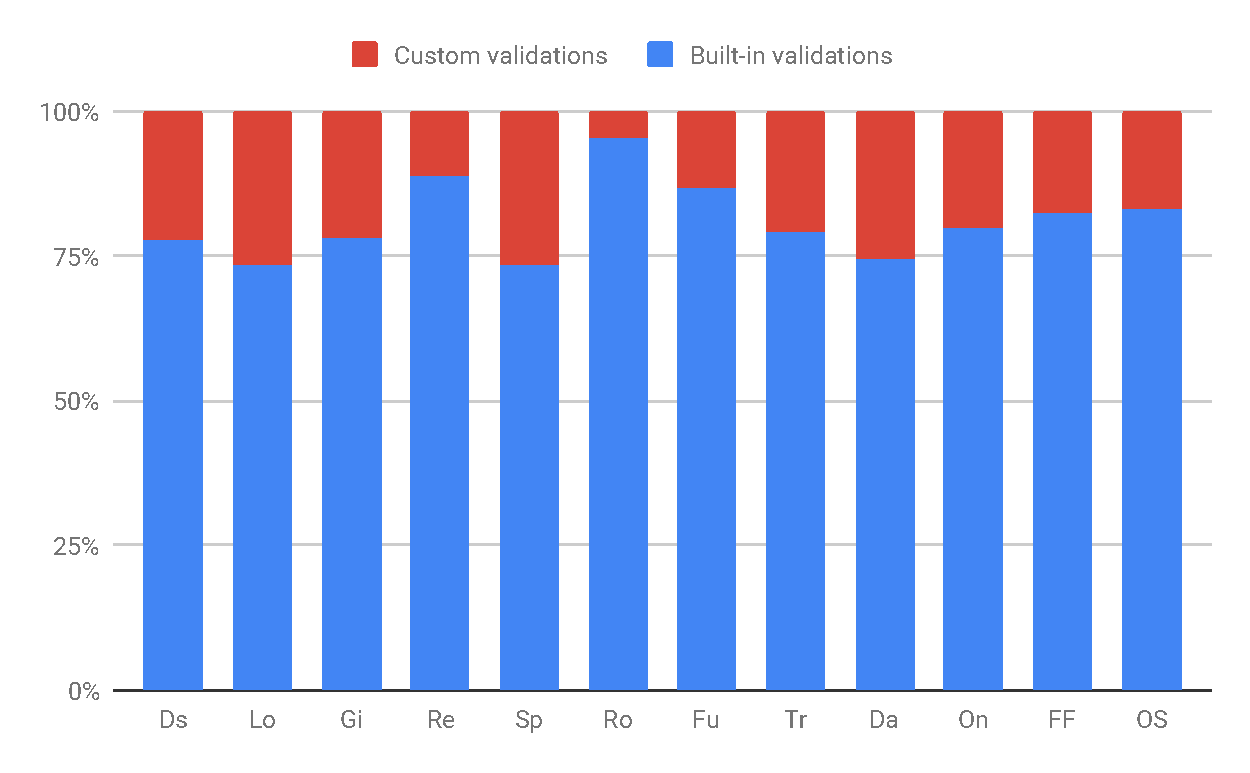
\includegraphics[width=\columnwidth]{figs/custom-vs-builtin-validations.pdf}
    \caption{Breakdown of \# of custom vs. built-in validations in model layer
\\  \junwen{change to a table?}
}
    \label{fig:model-breakdown}
\end{figure}
\fi 


\paragraph{\bf Custom sanity check types}

We also sampled 20 sanity checks on input parameters from the controller code of 5 applications.
%\shan{are these in one application or multiple? }
Among these 20 checks, the majority (17) are indeed checking inputs  that are related to persistent
data stored in the DB. Among these 17, 5 are about
data constraints, including presence and inclusion constraints, 
while the others are related to conditional data update/re-processing.
 Among these 5 constraints, only 1 is specified
in an application validation function and none exists in the DB.
%this 1 case is an inclusion constraint  

\iffalse 
\begin{table}[h]
\caption{\# Param sanity checking w/ category (sample size: 20)}
\footnotesize
\begin{tabular}{@{\hspace{0.1in}}r@{\hspace{0.2in}}r@{\hspace{0.2in}}r@{\hspace{0.2in}}r@{\hspace{0.1in}}}
\toprule
 Stored in DB & Constraint & Constrained in model & Constrained in DB\\
\midrule
17 & 5 & 1 & 0\\
\bottomrule
\end{tabular}
\label{table:nonapiconstraint}
\label{table:issueapp}

\end{table}
\fi 

\paragraph{\bf Summary} Although simple constraints like presence, length,
and numericality are the most common, more complicated constraints, such as those
involving multiple fields, are also widely used. Most of the
custom constraints are missing from the DB, while constraints reflected by sanity checks are often missing in both the application and DB. 
Future research that can automatically
reason about custom sanity checks and custom validation 
functions
%, which will likely require symbolic code evaluation,
can greatly help to identify and add missing constraints.

\section{Constraints   across versions}
\label{sec:evolve}

The software maintenance task for web applications comes with the
extra burden of database  maintenance, including both data format changes, 
like adding
or deleting a table column, and data constraint changes, like
changing the length requirement of a password field.
In this section, we study how constraints evolve across versions
and the related data-maintenance challenges.

\paragraph{\bf How often do constraint-related changes occur?} 
% As shown in  Table~\ref{table:firstlatestcomparison}, 
We first checked the first commit of each application, and found {\it no}
data constraints in all but 3 applications (Ds, Lo, FF).
For all applications, the majority of the constraints were added in later commits.

%We then check how often data constraints change across versions. 
%Different applications release software versions at different frequency: Gitlab has 7 releases within a single month\shan{is this average speed?}, while xxx \shan{give a slow example}. 
As shown in Table~\ref{table:percentage}, 21--95\% (avg. 49\% across all apps) of code versions contain
 data constraints that are different from those 
 in its previous version, 
 indicating that constraint changes are common. Note that, for
 most applications, we treat one code release as one version; for
 4 applications that do not specify release/version information,
 we treat every 100 code commits as one version.
 
 \begin{table}
\centering
% \setlength{\tabcolsep}{1.5pt}  
\caption{App. versions with constraint changes (\#Version$_\text{C}$)}
\resizebox{0.6\columnwidth}{!}{
%\begin{tabular}{l@{\hspace{0.1in}}r@{\hspace{0.1in}}r@{\hspace{0.1in}}r@{\hspace{0.1in}}r@{\hspace{0.1in}}r@{\hspace{0.1in}}r@{\hspace{0.1in}}r@{\hspace{0.1in}}r@{\hspace{0.1in}}r@{\hspace{0.1in}}r@{\hspace{0.1in}}r@{\hspace{0.1in}}r@{\hspace{0.1in}}}
\begin{tabular}{lrrrrrrrrrrrr}
\toprule
& {\color[HTML]{FE0000} Ds} & {\color[HTML]{000000} Lo} & {\color[HTML]{FE0000} Gi} & {\color[HTML]{FE0000} Re} & {\color[HTML]{FE0000} Sp} & {\color[HTML]{FE0000} Ro} & {\color[HTML]{000000} Fu} & {\color[HTML]{FE0000} Tr} & {\color[HTML]{FE0000} Da} & {\color[HTML]{FE0000} On} & {\color[HTML]{000000} FF} & {\color[HTML]{000000} OS}  \\ \midrule
\#Version & 316 & 19 & 1040 & 159 & 253 & 31 & 7 & 26 & 39 & 86 & 12 & 95 \\ \midrule
\#Version$_\text{C}$ & 187 & 18 & 563  & 44  & 89  & 20 & 4 & 12 & 26 & 18 & 10 & 41 \\ \midrule
\%Version$_\text{C}$  & 59\% & 95\% & 54\% & 28\% & 35\% & 65\% & 57\% & 46\% & 67\% & 21\% & 83\% & 43\% \\ \bottomrule
\end{tabular}
}

\label{table:percentage}
\footnotesize{All types in Table \ref{table:constraintdeftax} except for custom sanity checks are considered.\\Red apps use a release as a version; Black apps use every 100 commits as a version.}
{\footnotesize }
\end{table}

 
\iffalse 
\begin{table}

\setlength{\tabcolsep}{2pt}  
\caption{\# Data constraints in the first and the latest version}
\resizebox{0.7\columnwidth}{!}{
\begin{tabular}{lrrrrrrrrrrrr}

\toprule
& Ds   & Lo  & Gi   & Re  & Sp  & Ro  & Fu & Tr  & Da  & On  & FF  & OS  \\
\midrule
first & 181 & 66 & 0 & 0 & 0 & 0 & 0 & 0 & 0 & 0 & 13 & 0\\
\midrule
latest  & 1764 & 160 & 1970 & 693 & 131 & 594 & 47 & 142 & 482 & 453 & 177 & 413 \\
\bottomrule
\end{tabular}
}
\label{table:firstlatestcomparison}
\footnotesize{All types in Table \ref{table:constraintdeftax} except for custom sanity checks are considered.}
\end{table}
\fi 

% \begin{table}[h]
% \caption{App. versions with constraint changes (\#Version$_\text{C}$)}
% \resizebox{\columnwidth}{!}{
% \begin{tabular}{l@{\hspace{0.1in}}r@{\hspace{0.1in}}r@{\hspace{0.1in}}r@{\hspace{0.1in}}r@{\hspace{0.1in}}r@{\hspace{0.1in}}r@{\hspace{0.1in}}r@{\hspace{0.1in}}r@{\hspace{0.1in}}r@{\hspace{0.1in}}r@{\hspace{0.1in}}r@{\hspace{0.1in}}r@{\hspace{0.1in}}}
% \toprule
% & Ds & Lo & Gi & Re & Sp & Ro & Fu & Tr & Da & On & FF & OS\\
% \midrule
% \#Version & 339 & 19 & 949 & 144 & 197 & 18 & 7 & 39 & 196 & 83 & 12 & 91 \\
% \midrule
% \#Version$_\text{C}$ & 177 & 15 & 173 & 65 & 66 & 15 & 4 & 19 & 77 & 11 & 11 & 27\\
% \midrule
% \%Version$_\text{C}$ & 52\% & 79\% & 18\% & 45\% & 34\% & 83\% & 57\% & 49\% & 37\% & 13\% & 92\% & 27\%
% \\
% \bottomrule
% \end{tabular}
% }
% \label{table:issueapp}

% {\footnotesize }
% \end{table}

% \junwen{the new table of release is saved at tables/percentageofchangedrelease.tex}

 \paragraph{\bf What triggered changes?}
We categorize all the cross-version changes about DB constraints
and application validation constraints into three types: 
(1) Add Column: adding constraints to a data column that did not exist in previous version;
(2) Add Constraint: 
adding constraints to an existing data column that was not associated
with that specific type of constraints, like adding a length
constraint to a data field that had no length constraint previously;
(3) Change Constraint: changing the detailed requirement of a constraint that already
existed in previous version.

% \shan{do these applications really no have public release versions?
% is it possible that the multiple versions here actually belong to the same
% public release?} \junwen{8 applications have release versions}


%Ideally, most constraint changes should belong to the Add-Column type, which would indicate stable and timely constraint maintenance. However, this is often not true ---
What is alarming from the result (Figure~\ref{fig:constraints-num})
is that the Add-Column type only 
contributes to around or lower than 50\% of changes in 
5 out of the % data source: https://docs.google.com/spreadsheets/d/1h8LZAczQoTkSXWalqBymrRVKCTxuxaH946snlQDnRwk/edit?usp=sharing 
12 applications. On the other hand, 13--67\% of constraint changes
(23\% across all applications) are adding new types of constraints to columns that already existed in earlier versions (i.e., tightening the constraints),
indicating that constraint addition is often developers' after-thoughts.
Changing existing constraints is much less common, but is still not rare, contributing to more than 10\% of constraint
changes in 4 applications.
% \shan{Junwen, pls change figure 2,
% so that its height is this short, but the in-figure caption is more readable?}
% Lobsters, gitlab, diaspora
 


\begin{figure} 
    \centering
    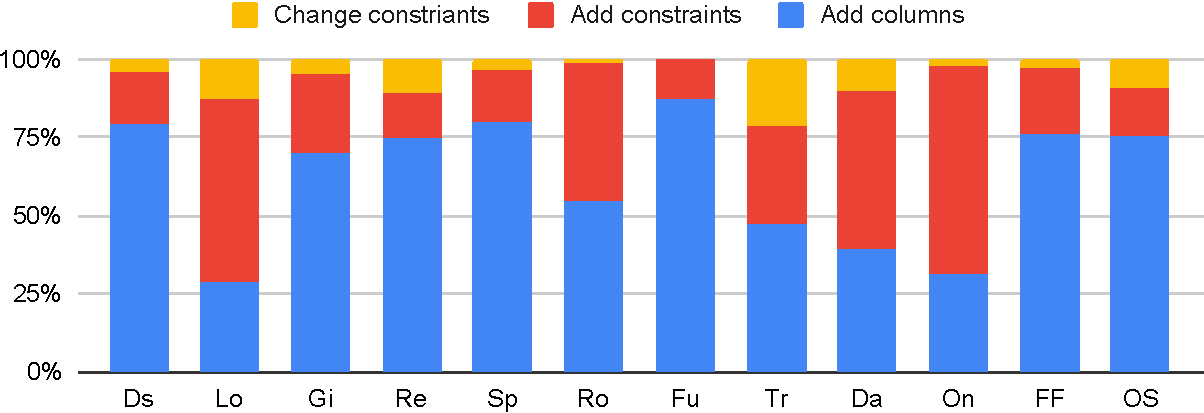
\includegraphics[width=0.6\columnwidth]{constraints//figs/breakdown-release.pdf}
    \caption{Breakdown of \# of adding/changing constraints 
\\   
%\junwen{the figure of release unit is saved as figs/breakdown-release.pdf}
}

    \label{fig:constraints-num}
\end{figure}


\paragraph{\bf Summary} It is problematic
that around or more than a quarter of constraint-related code changes in
most applications are about adding constraints to already existing data columns. This indicates a widely existing vulnerability that allows constraint-violating data to be stored into the database before the correct constraints are imposed. 
Tools are needed to help developers add 
suitable constraints whenever a new data column is created and 
warn of data that is incompatible with the newly added constraints.
  

% \begin{figure}[h]
%     \centering
%     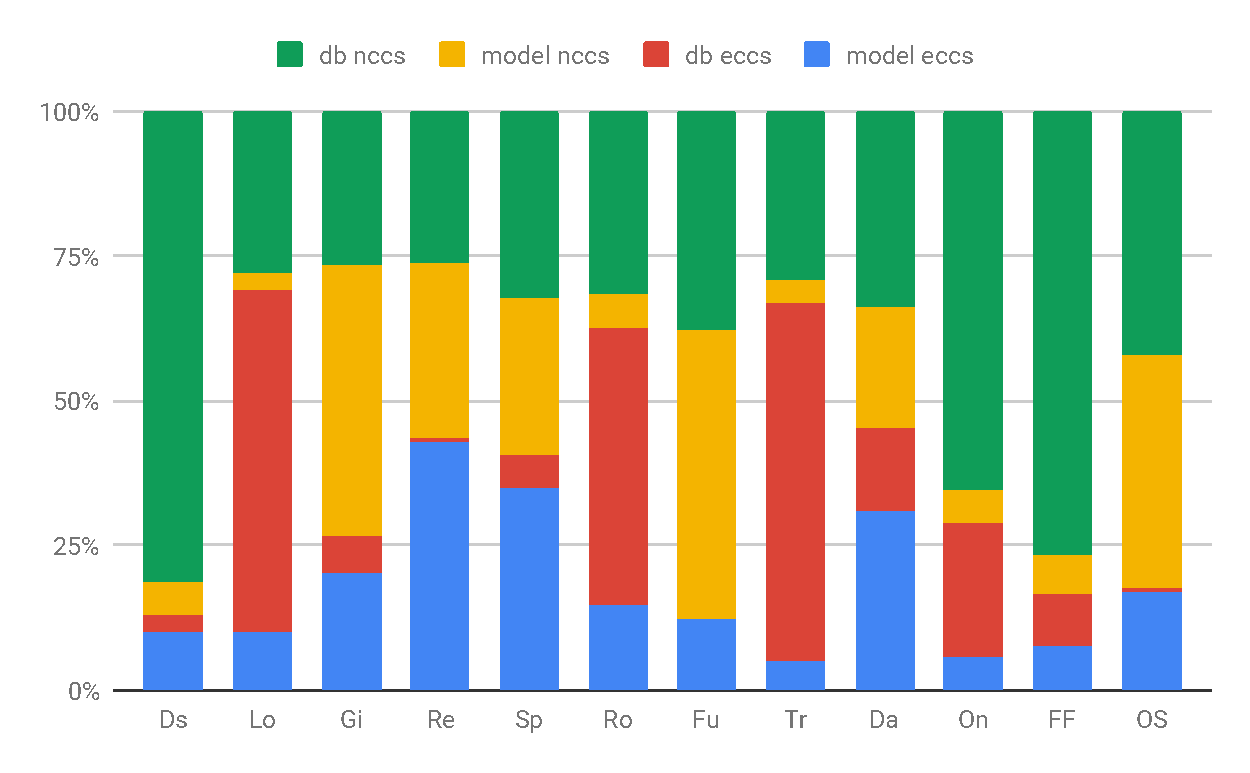
\includegraphics[width=\columnwidth]{figs/existing-new-columns.pdf}
%     \caption{Breakdown of \# of constraints on new/exsiting columns}
%     \footnotesize{nccs: adding constraints on new columns; 
%     eccs: 
%     adding constraints on existing columns}
%     \label{fig:exist-column}
% \end{figure}


% Later
% \begin{figure}[h]
%     \centering
%     \includegraphics[width=\columnwidth]{figs/total.pdf}
%     \caption{Trend of Changing/adding constraints towards line of code change\shan{???first, may want to draw the figures in a different way; second, if absolutely no trend, not worth the space}}
%     \label{fig:exist-column}
% \end{figure}

\section{Constraint-related issues}
\label{sec:causes}
% After studying the \numissues data constraint issues reported in the applications' bug-tracking systems, 
 We categorize \numissues real-world issues 
 into 4 types as shown in Table \ref{tab:issuecat}.
 
 \iffalse 
 :
 (1) data constraints located at different software components conflict with
 each other (WHERE issue); (2) the exact requirement imposed by a data constraint
 conflicts with what the users or the application logic actually expects 
 (WHAT issue); (3) data constraints specified in different code versions conflict
 with each other (WHEN issue); and (4) a constraint's violation-checking result
 is not properly delivered to web users (HOW issue).
 \fi 



\subsection{WHERE is the constraint specified?}
\label{subsec:where}
As discussed, application and DB constraints for the same data field can be inconsistent with each other. Such inconsistencies contributed to 24 out of the 114 issues.

\paragraph{\bf Application constraints looser than DB constraints} 13 out of 24 issues fall into this category. In 12 of them, the constraint is completely missing in application layer while the rest one issue happens because the length constraint has a smaller value in database layer than in application layer.
In these cases, a record saving operation would pass the application server's
checking but fail in the DB, causing a web page crash
with an unhandled raw DB error thrown to end users, which is
often difficult to understand and causes poor user experience. The example discussed in 
Figure \ref{fig:crossstack} is an illustration. 

\paragraph{\bf Application constraints stricter than DB constraints} 11 out of 24 issues fall into this category. In 9 of them, application constraints are not defined in database layer at all while the rest two are caused by that length constraint has smaller value in application layer than in database layer.  
In these cases, the application misbehaves as the administrator/user
directly 
%\shan{who exactly can issue SQL request to DB server directly?}
changes database records through SQL queries in a way that violates application constraints. This happens quite often.   For example, Spree \cite{spree}, an on-line shopping system, has 4 issues caused by administrators modifying database content through direct SQL requests. Discourse \cite{discourse} even has scripts that bypass model constraints to import other forum applications' data. 

Figure~\ref{fig:spree-3829-different} shows such an issue~\cite{spree-3829} in Spree. As shown in (b), each {\tt LineItem} is associated with a {\tt variant} object and a {\tt presence} constraint is used to ensure the existence of every associated {\tt variant}. This ensures that an expression like
{\tt item.variant.image} in (a) is never null.
%Specifically, this presence constraint is checked whenever an {\tt LineItem} object is saved by the application, and it would cause the saving to fail if the associated {\tt variant} object does not exist. 
However, this constraint does not exist in the database. In this bug report,
an adminstrator accidentally deleted a {\tt variant} record in the DB
that is associated with a {\tt LineItem} record, and that
led to a null pointer error when he tried to display 
an order through the code in Figure~\ref{fig:spree-3829-different}a. 
%In the spree issue, only admin users will be affected by the corrupted data. However, there are other issues such as Discourse-30278 in which normal users suffer from null-pointer errors with page crashes because one post's topic has been deleted. 

\begin{table}[]
\centering
\caption{Data-constraint issues in real-world apps}
\label{tab:issuecat}
\setlength{\tabcolsep}{4pt}  
\resizebox{0.6\columnwidth}{!}{
% \begin{tabular}{lrrrrrr}
% \toprule 
% & WHERE
% &  \multicolumn{2}{c}{WHAT}   & WHEN  & HOW & SUM  \\ 
% \cmidrule{3-4}
% & 
% &  vs. code  & vs. user  &   &  &   \\ 
% \midrule
% Ds  & 3  & 0  & 6  & 2  & 2  & 13  \\ \midrule
% Lo  & 0  & 1  & 0  & 0  & 0  & 1   \\ \midrule
% Gi  & 3  & 8  & 0  & 4  & 1  & 16  \\ \midrule
% Re  & 7  & 11 & 4  & 1  & 7  & 30  \\ \midrule
% Sp  & 8  & 14 & 3  & 3  & 3  & 31  \\ \midrule
% Ro  & 0  & 1  & 1  & 0  & 0  & 2   \\ \midrule
% Fu  & 1  & 0  & 0  & 0  & 0  & 1   \\ \midrule
% Tr  & 0  & 0  & 1  & 1  & 0  & 2   \\ \midrule
% Da  & 0  & 4  & 1  & 1  & 5  & 11  \\ \midrule
% On  & 2  & 2  & 1  & 0  & 0  & 5   \\ \midrule
% FF  & 0  & 0  & 0  & 0  & 0  & 0   \\ \midrule
% OSM & 0  & 0  & 0  & 0  & 2  & 2   \\ \midrule
% SUM & 24 & 41 & 17 & 12 & 20 & 114 \\ \bottomrule
% \end{tabular}

\begin{tabular}{@{}rrrrrrrrrrrrrrr@{}}
\toprule
                      &          & Ds & Lo & Gi & Re & Sp & Ro & Fu & Tr & Da & On & FF & OSM & SUM \\ \midrule
WHERE                 &          & 3  & 0  & 3  & 7  & 8  & 0  & 1  & 0  & 0  & 2  & 0  & 0   & 24  \\ \midrule
\multirow{2}{*}{WHAT} & vs. code & 0  & 1  & 8  & 11 & 14 & 1  & 0  & 0  & 4  & 2  & 0  & 0   & 41  \\ \cmidrule(l){2-15} 
                      & vs. user & 6  & 0  & 0  & 4  & 3  & 1  & 0  & 1  & 1  & 1  & 0  & 0   & 17  \\ \midrule
WHEN                  &          & 3  & 0  & 4  & 1  & 3  & 0  & 0  & 0  & 1  & 0  & 0  & 0   & 12  \\ \midrule
HOW                   &          & 2  & 0  & 1  & 7  & 3  & 0  & 0  & 0  & 5  & 0  & 0  & 2   & 20  \\ \midrule
SUM                   &          & 14 & 1  & 16 & 30 & 31 & 2  & 1  & 1  & 11 & 5  & 0  & 2   & 114 \\ 


\bottomrule
\end{tabular}
}
\footnotesize{}
\end{table}


\begin{figure}
    \centering
    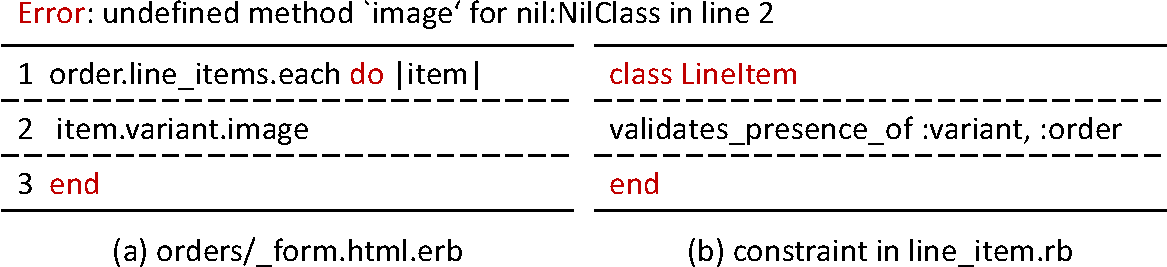
\includegraphics[width=0.6\columnwidth]{constraints/figs/spree-3829-different2.pdf}
    
    \caption{Constraint mismatch in Spree}
    
    \label{fig:spree-3829-different}
\end{figure}

% The could also be incompatibility between html layer and model 

% \junwen{We don't have issues caused by inconsistency of html constraint and model constraint. If there is, the symptom would be  misleading error message. }
% \shan{I remember you started looking into html-end constraint because you saw some
% inconsistency. right?}

\paragraph{\bf Summary}
As shown by real-world issues, inconsistencies between application 
 and database constraints cause problems, including
web page crashes and poor user experience.
Considering the hundreds and thousands of constraints that exist in the DB
but not in application and vice versa 
(see Section~\ref{sec:one_where}), 
this problem could be much more severe and widespread than
what reflected by the issue reports.
Automatically detecting such constraint inconsistencies will be very helpful, which we further explore in Section \ref{sec:solution}.

\subsection{WHAT is the constraint about?}
\label{subsec:what}
The most common problem is a mismatch between how data is supposed to be used in the application and the constraints imposed on it. This accounts for 
58 out of \numissues issues. 
%\alvin{i don't quite get what you mean. you mean conflict between constraints specified in app vs constraints specified in the db?}\shan{no, it is like the constraint said this should be an integer, but the application tries to get the square root of this data, which indicates the constraint should positive-integer, not just integer.}


\subsubsection{{Conflict with user needs}}

Users sometimes would relax an existing constraint,
such as increasing the input length of name field in tracker from 30 to 100 (Redmine-23235 \cite{redmine-25235}).
These contribute to about 10\% of the issues in our study.
%Another user in Tracks asks ``The passwords are limited to 40 characters.
%I don't like the limit, so is it possible to increase it?''. 
%The solution is simple as shown in Figure~\ref{fig:tracks-1921-passwordlength}, 
%in Discourse-79684: ``On our site users sometimes want really long `About Me' descriptions in their profiles but it is by default limited to 3000 characters. Is there any easy way to bump this up?''.
%Similarly, a user posted an issue in Discourse \cite{discourse.75453}, saying ``Does anyone know if there is a way to modify the maximum character limit for category names? I need to ...".
%put an English title, followed by the French equivalent, but I am running out of room to do both.''. 
Developers usually satisfy the users' desires and change constraints
accordingly. 

\iffalse
In Redmine, the corresponding length-constraint was only
specified in application, not in DB, and the patch simply changed
the application validation function parameter to allow longer
inputs; in Discourse, since Category-name has its length constraint
specified in both application and in DB, the patch changed
both places.
\fi 

% Sometimes, the constraints validation needs to be skipped. For example, in Spree-7389, user says ``There is validation for Address model for zipcode. It's always check it even though this may be problem because for example Hong Kong doesn't have zipcodes.''

\iffalse 
\begin{figure}
    \centering
    \includegraphics[width=0.8\columnwidth]{figs/tracks-1921-passwordlength.pdf}
    \caption{Too tight constraint in Tracks}
    \label{fig:tracks-1921-passwordlength}
    %link: https://github.com/TracksApp/tracks/issues/1921
\end{figure}
\fi 

\paragraph{\bf Summary}  For certain type of constraints, like the
length constraint, it is difficult to have one setting that satisfies all users' needs. It would be helpful if refactoring routines can be designed to turn a fixed-setting constraint into configurable. %\shan{1.none of your example above is about configurable; 2.it is better to suggest some automation, like suggesting refactoring that makes some constraints that involve numerical bounds to be user configurable.}. 


\subsubsection{{Conflict with application needs}}
\label{sec:what_app}
Many constraints are created to guarantee program invariants
that are crucial to applications' functional correctness. 
Constraints that are insufficient or even conflicting with how the corresponding
data is used by the application contribute to more than one third of all the issues
in our study.

\paragraph{\textbf{Type conflicts}}
These constraints treat a data field as having a general type, but
the application uses the data field in a more specialized way
that demands tighter constraints. In one Redmine issue~\cite{redmine-9394}, a user noticed that she can input  invalid dates like
``2011-10-33'' without triggering any errors. 
This problem happened because Redmine only used a regular expression ``\textbackslash d\{4\}-\textbackslash d\{2\}-\textbackslash d\{2\}\textdollar'' to make sure the input follows the ``yyyy-mm-dd'' format without more detailed checking.
To solve this problem, Redmine later added ``value.to\_date'' to check whether the input   can really be converted to a date or not in the custom validate function shown in Figure~\ref{fig:redmine-9394-tooloose}.  

\begin{figure}
    \centering
    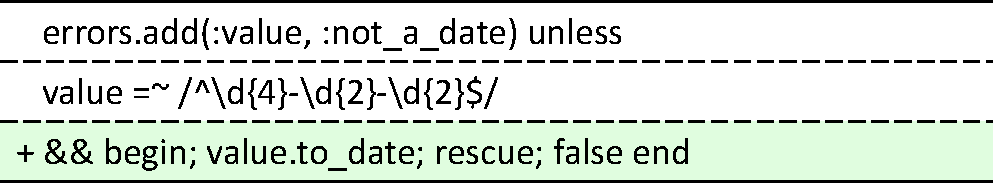
\includegraphics[width=0.6\columnwidth]{constraints/figs/redmine-9394-tooloose.pdf}
    \vspace{-0.2in}
    \caption{Type conflict example in Redmine}
    %\vspace{-0.1in}
    \label{fig:redmine-9394-tooloose}
\end{figure}

\textbf{Case sensitivity conflicts.} 
{\it Uniqueness} is a common constraint associated with a data field to
avoid duplication, like preventing two users from having the same ID. 
A common problem is that a field is written to the DB in
a case-sensitive way of uniqueness, while used or searched in a
case-insensitive way, or vice versa. Such inconsistency can lead to severe software misbehavior. 

In a Gitlab issue~\cite{gitlab-24493}, a user's profile email is all in lower case, but she committed code with an upper-case letter in her email, which then cannot
be matched to her profile. What is annoying was that she was 
unable to add the different casing as an alias, as Gitlab said
the email was ``already in use.''  This happens because when a user-email is stored into DB, the uniqueness checking
is case insensitive---``abc@example.com'' is treated the same as ``ABC@example.com.'' However, when the application searches for code commit using email
as the index, the search is case sensitive --- code committed by
``ABC@example.com'' cannot be retrieved by a search using
``abc@example.com.'' The patch made the search also
case insensitive, thus always converting the input email to pure-lowercase before the
search, as shown in Figure~\ref{fig:gitlabcasesensitive}. 

\begin{figure}
    \centering
    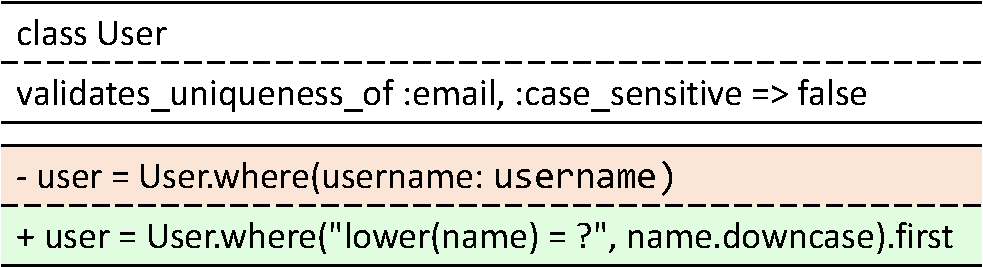
\includegraphics[width=0.6\columnwidth]{constraints/figs/gitlab-issue.pdf}
    \caption{Case sensitivity conflict example in Gitlab}
    %\vspace{-0.1in}
    \label{fig:gitlabcasesensitive}
\end{figure}

\textbf{Boundary value conflicts.} There are cases where certain
values of a data field are allowed by the application logic, 
but disallowed by the constraints. For example, in the typical checkout flow of Spree, users would enter their delivery details, then proceed to a payments page to enter discounts and payment details, and then finally arrive at a confirmation page. However, in one Spree issue\cite{spree-6673}, a user complained that when she entered a discount coupon that reduced the price to zero---which was actually a valid use case---the application did not allow him to proceed, and instead redirected back to the delivery page. The source of the bug was a constraint in the model layer ({\tt models/spree/order.rb}) which
%, in order to proceed to the next stage of the checkout flow, 
incorrectly required the value of the {\tt total} field to be strictly greater than zero.

\iffalse 
\begin{figure}
    \centering
    \includegraphics[width=\columnwidth]{figs/spree-issue.pdf}
    %\vspace{-0.1in}
    \caption{Boundary value inconsistency in Spree}
    \label{fig:spreerwinconsistency}
\end{figure}
\fi 

\paragraph{\bf Summary}
Failure symptoms of these bugs are quite different from all the other types 
of bugs (WHERE, WHEN, HOW). They can lead to severe software misbehavior or even
disable an entire feature of a web application.  
It would be ideal if a program analysis tool can compare how a data field
is used in software and identify inconsistency between how it is used and 
how it is constrained. This is challenging for generic data
types and data usage, but is feasible for specific types of 
problems, which we explore
in Sec. \ref{sec:solution}.


\subsection{WHEN is the constraint created?}
\label{subsec:when}

When upgrading an application, sometimes newly added or changed constraints might be incompatible with old data. 
12 issues are caused by such inconsistency across versions. 
The failure symptoms vary based on the different program context where the 
tighter constraint is checked.

\paragraph{\textbf{Read path}}
When a constraint is newly created or tightened along a DB-record loading code
path (e.g., front-end
constraint or application sanity-check changes), an  
incompatible new constraint can cause failures in
loading old data and hence severe functionality problems.
The Diaspora example in Section~\ref{sec:intro} belongs to this
category: the password's length requirement tightened and hence invalidated many old passwords.

\iffalse 
In the old version of Diaspora, it is allowed to set the password with length smaller than three. In one commit, developers have added an constraint in HTML level with format ``......+'' which limits the password  to be equal or longer than 6 characters. This causes many users, whose
passwords are shorter than 6 character, to fail to login to Diaspora with the 
unhelpful error-information saying ``Please use the required format''. 
Their solution is to remove the newly added constraints on the password length.


\begin{figure}
    \centering
    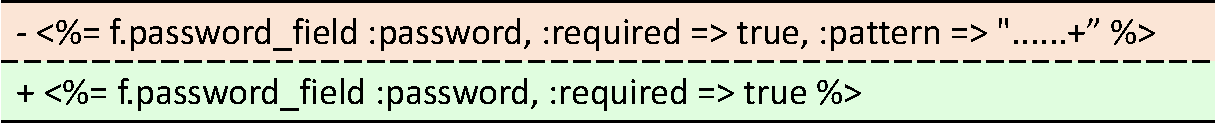
\includegraphics[width=\columnwidth]{figs/diaspora-4221-password.pdf}
    \vspace{-0.2in}
    \caption{Old data conflicts with new constraints (Diaspora)}
    \label{fig:diaspora-4221-password}
\end{figure}
\fi 

\paragraph{\textbf{Write path}}
When a constraint is newly created or tightened along a path that intends to
save a record to the database (e.g., all the application-validation constraints
and database constraints), the incompatibility between the new constraint
and old data can be triggered under the following two circumstances.
 

First, all the old data in the database will be checked against the new set 
of DB constraints during a migration process during
application upgrade. 
Inconsistency between old data and new DB constraints can cause an upgrade failure.
For example,
one Gitlab issue~\cite{gitlab-36919} complains that they failed to upgrade from version 9.4.5 to 9.5.0 due to {\tt NotNullViolation} during data migration. As shown in Figure~\ref{fig:gitlab-36919-when}, the {\tt decription\_html} column was added 
to Gitlab before version 9.4.5 (in the ``20160829...'' migration file) and was filled with {\tt null}s by 
default.\footnote{When no default value is specified in {\tt add\_column}, {\tt null} is used as the default value.}
% in migration add\_markdown\_cache\_columns.rb before 9.4.5, but the column still has null value
Later on, in the ``20170809...'' migration (shown in the Figure~\ref{fig:gitlab-36919-when}), a non-null constraint 
was added to the column through the API {\tt change\_column\_null} with parameter {\tt false}. This caused 
many users' upgrade to fail because there were many old records with
a default {\tt null} in that column. 
%There are two solutions to solve this issue, one is to change the constraint, 
The patch removed the ``non null'' constraint to the {\tt description\_html} column, as shown in 
Figure~\ref{fig:gitlab-36919-when}. 
%Of course, an alternative solution is to set a not-null default value for the column as shown in Figure~\ref{fig:gitlab-36919-when}.
%--edit to here
%We have also seen cases where the migration file added a new column with a {\tt not-null} constraint without setting default value for it. As a result, the system by default fills the new column with {\tt null} and immediately leads to migration/software-upgrade errors such as that in Gitlab-46862. 


Second, even if all the old data is validated against DB constraints and the application has successfully upgraded, the old data might still conflict
with new constraints specified through the application validation APIs that did not exist in the prior version.
This can lead to problems when the application allows users to edit an existing
 record---users may have trouble in saving an edited record back.
In one Discourse issue~\cite{discourse-89148}, a user complained that she made a small edit to an old post's  title, but was unable to save with an error message stating that the title was invalid.
It turned out that, the 
title's length constraint has been changed from 30
 to 20 characters in the application's validation function. That old post's title contained
28 characters; the small edit did not change the title length. So, the old post can still be loaded by the application, but cannot be saved back after such small edits.
 

 

\begin{figure}
    \centering
    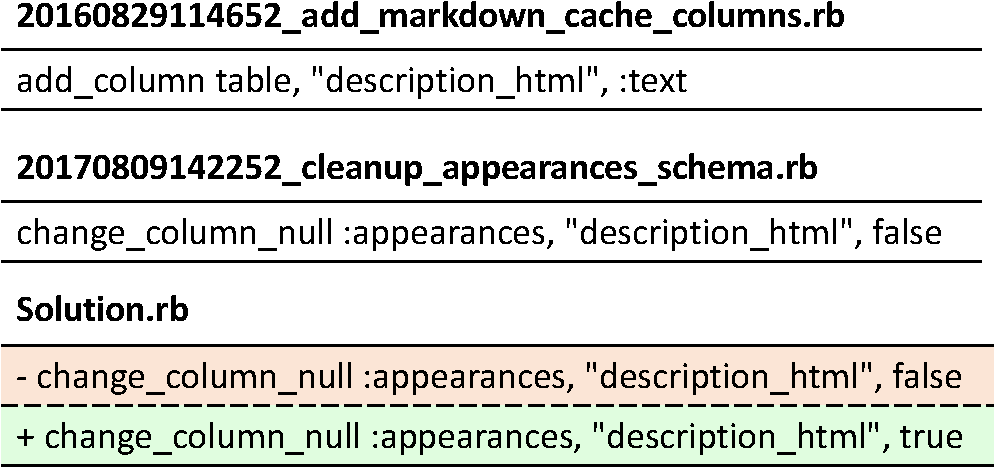
\includegraphics[width=0.6\columnwidth]{constraints/figs/gitlab-36919-when.pdf}
    \caption{Old data conflicts with new constraints in Gitlab}
    %\vspace{-0.1in}
    \label{fig:gitlab-36919-when}
\end{figure}

\paragraph{\bf Summary}  Given the frequent constraint addition and changing
in web applications, it is inevitable that old data may
become incompatible with new constraints. It would be helpful if automated 
tools can provide warnings for developers when constraints become
tighter in a new version, particularly (1) if the migration file has high probability to
fail (e.g., specifying a constraint that conflicts with a column's default value), then developers should fix the migration
file; (2) if the application allows editing old data, then developers should probably 
add explicit warning to users about the risk of editing old data; and finally
(3) the case of having tighter constraints that limit the reading of old data should be avoided. We explore this in Section~\ref{sec:solution}.

\subsection{HOW are the checking results delivered?}
%\utsav{Possibly include results on what portion of custom validations might be missing errors}
\label{subsec:how}

Constraint violation is common in web applications, as web users cannot anticipate all the constraints
in advance and will inevitably input constraint-violating data. Consequently,
delivering informative and friendly error messages is crucial to web applications'
user experience. 20 issues in our study are about this problem. 
 
These 20 issues are mostly related to application-validation constraints.
Rails validation APIs provide default error messages that are mostly 
clear.\footnote{Section~\ref{sec:solution} discusses cases when the default message is unclear
and how we enhance it.} However, developers 
sometimes forgot to display the error message associated with the validation
APIs (8 cases) and sometimes override the default message with
uninformative generic messages (12 cases), which led to user complaints.
For example,
in a Diaspora issue~\cite{diaspora-5090}, a user complained that when he tried to post a long article, the posting failed with an unhelpful error message ``Failed to post!'' 
%The user demanded ``a more descriptive error message''. 
Developers found out that their code in {\tt posts\_controller} forgot to render the error message
defined in {\tt post}'s validation function. The patch fixed this problem
and would display the required length limit,
as shown in Figure~\ref{fig:diaspora-5151-errormsg}.
%\shan{Junwen, please make the patch figure simpler, only
%reflecting the change to show the length limit.}
%by ``please make your post less than 65536 characters''. Although this is not the default error message provided by Rails, the information revealed is the same. 
%In this particularly case, users later further requested to know not only the post limit but also the length of their failed submission, which was satisfied by later patches. 
%So eventually the error message was changed to ``Please make your post fewer than 65536 characters. Right now it is \%\{length\} characters'', in which  \%\{length\} is the current length of users' input post.
\begin{figure}
    \centering
    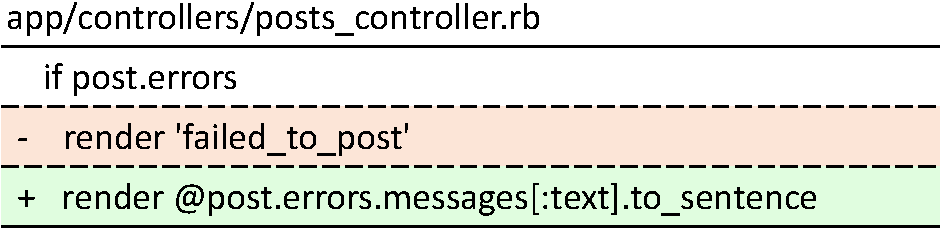
\includegraphics[width=0.6\columnwidth]{constraints/figs/diaspora-5990-errormsg-cp.pdf}
    \caption{Unclear error message in Diaspora}
    \label{fig:diaspora-5151-errormsg}
    %link: https://github.com/diaspora/diaspora/issues/2481
\end{figure}

\paragraph{\bf Summary} Developers should be reminded to display error messages associated with validation APIs. Future IDEs should automatically 
synthesize default error checking and error-message display code. 
Improving the quality of default and custom error message is crucial to
user experience. We will explore this in Section~\ref{sec:solution}.
%Some issues however requires a better understanding of the application behavior facing errors.
 

% \iffalse
% In Diaspora-2481, many users complain that they tried many times to reset password but failed with a bunch of error messages as shown in Figure~\ref{fig:diaspora-2481-unclear}~(b), which is very confusing since in the password reset page, there are only two fields for the new password and confirmation of it. There is no email and username on that page at all, not to mention the error message. The developer figured out this happens because the email address has been invited to Diaspora, but hasn't accepted the invitation yet, which is not reflected through the error message at all. And do not underestimate the importance of the error message. They are crucial to the popularity of the applications. A user says ``I had no idea what those messages meant, and a normal user would simply abandon their account.''. \shan{yeah, this
% bug is interesting. However, are we doing anything to help resolve this problem?
% the problem here seems to be that the error message is complaining about a field
% that the user entered in a previous page, right? That seems to be different
% from the problem you guys worked on?}

% \begin{figure}
%     \centering
%     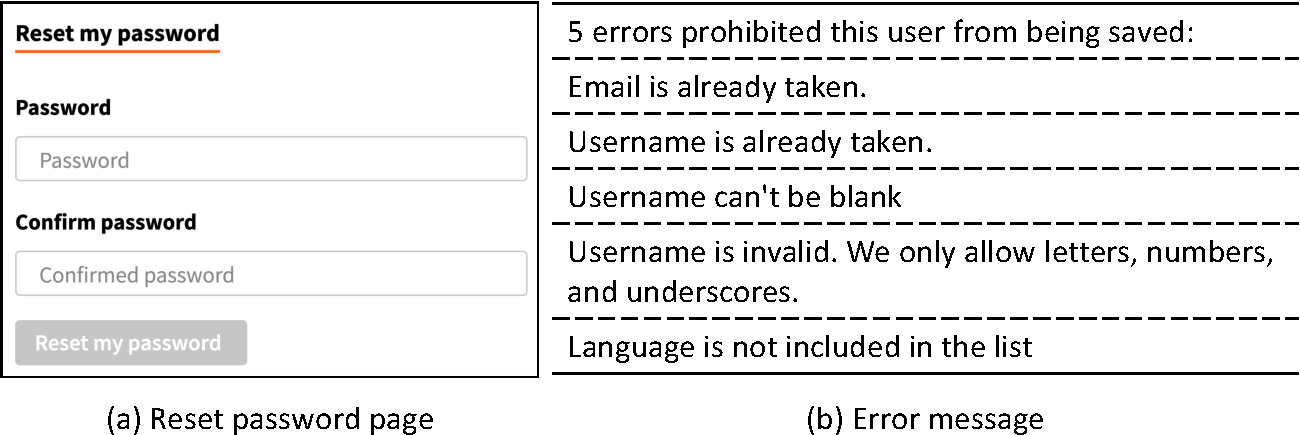
\includegraphics[width=\columnwidth]{figs/diaspora-2481-unclear.pdf}
%     \caption{Unclear error message in Diaspora}
%     \label{fig:diaspora-2481-unclear}
%     %link: https://github.com/diaspora/diaspora/issues/2481
% \end{figure}

% \endif

 \section{Solutions \& Evaluation}
\label{sec:solution}
  
%Guided by the patterns discussed above, we explore detecting some of these problems  in the {\bf latest} versions of these 12 applications. 

We now discuss our experience in building tools to automatically discover the anti-patterns discussed earlier. We focus on applying them to the latest versions of the studied applications, as these represent potential bugs that have not been discovered.

\subsection{Where issues}

As discussed in Section~\ref{sec:one_where}, our scripts can automatically find more than 1000 string-length DB constraints that are missing in application, and more than 400 application built-in-validation constraints
 that are missing in the DB. We reported 16 of them covering different types, with 12 of them already confirmed by developers from 3 applications (Lo, Ds, FF).

In addition, we extended our scripts to automatically find conflicting cases, where
the same type of constraint, like length, is specified for the same 
data field in both database and application, but the exact constraint requirement is different.

As shown in Table~\ref{table:mismatchdbmodel}, our checker reported 138 conflicting constraints in total.
Our manual checking confirmed that 133 of them are true conflicts and 5 are false positives.

These 133 conflicts include 84 cases where
applications' length constraints are tighter than the DB's, 4 cases in the other way, 1 case where the columns referenced by uniqueness constraints did not exactly match, and 44 cases where the range or type of numeric values allowed in DB did not match the corresponding restriction in the model. 
For example, our results showed that, in the Tracks application, there was a string field {\tt description} in model {\tt Todo} for which the length in DB was limited to 255 characters, but was limited to 300 in the model. 
%This would cause requests to fail if a user entered a description between these two lengths. 
We reported this mismatch to developers and received confirmation that it was indeed a bug. 
As another example, we found 5 instances in OpenStreetMap where developers meant to require 
fields to be integers in both the DB and application. However, developers had typos in their use of validation APIs, which caused the application-level numericality constraints to be silently ignored. 
We reported this to developers, who then fixed the bug.

% \begin{table} 
\setlength{\tabcolsep}{3pt}  
\caption{\# Reported Issues}
\resizebox{\columnwidth}{!}{
\begin{tabular}{lrrrrrrrrrrrr}

\toprule
& Ds   & Lo  & Gi   & Re  & Sp  & Ro  & Fu & Tr  & Da  & On  & FF  & OS  \\
\midrule
Reported & 5 & 6 & 0 & 1 & 0 & 0 & 0 & 1 & 1 & 0 & 3 & 20 \\
\midrule
Confirmed & 2 & 6 & 0 & 0 & 0 & 0 & 0 & 1 & 1 & 0 & 3 & 20 \\ 
% data source https://docs.google.com/spreadsheets/d/1d9wh0BxLLgQaSKSxFTA3ou5RH7P5D8LKaHQ1paU45u8/edit?usp=sharing
\bottomrule
\end{tabular}
}
\label{table:reportedissues}
\end{table}

% Table~\ref{table:reportedissues} shows the detailed number of our reported and confirmed issues. 


%\shan{do you have any good value range example?}\utsav{Pretty much any time a developer specifies a range in model, this results in mismatch, because no explicitly-defined ranges exist in DB layer (i.e. it is always implicit [INT\_MIN, INT\_MAX]). Example follows but we do not report anything because we have no clear solution.} 
As an example of range mismatch, there was a case in Spree where the field {\tt price} must be greater than or equal to zero. However, in the DB, the field type was {\tt decimal} which allows negative values.

Among the 5 false positives, 3 were caused by our tool's limited ability in handling non-literal expressions, and the others were related to our tool's inability to distinguish between array length and string length validations.

\begin{table} 
\centering
\setlength{\tabcolsep}{3pt}  
\caption{\# Mismatch constraints between DB-Model}
\resizebox{0.7\columnwidth}{!}{
\begin{tabular}{lrrrrrrrrrrrr}

\toprule
& Ds   & Lo  & Gi   & Re  & Sp  & Ro  & Fu & Tr  & Da  & On  & FF  & OS  \\
\midrule
Length - DB looser & 5 & 7 & 12 & 9 & 0 & 25 & 0 & 4 & 4 & 11 & 0 & 7\\
\midrule
Length - DB tighter  & 0 & 0 & 0 & 0 & 0 & 3 & 0 & 1 & 0 & 0 & 0 & 0 \\
\midrule
Uniqueness  & 1 & 0 & 0 & 0 & 0 & 0 & 0 & 0 & 0 & 0 & 0 & 0 \\
\midrule
Numericality  & 4 & 0 & 24 & 1 & 6 & 0 & 3 & 0 & 0 & 0 & 3 & 3 \\
\midrule
{\it False positives}  & 0 & 0 & 2 & 3 & 0 & 0 & 0 & 0 & 0 & 0 & 0 & 0 \\
\midrule
Total  & 10 & 7 & 38 & 13 & 6 & 28 & 3 & 5 & 4 & 11 & 3 & 10 \\
% \midrule
% Reported & 5 & 6 & 0 & 1 & 0 & 0 & 0 & 1 & 1 & 0 & 3 & 20 \\
% \midrule
% Confirmed & 2 & 6 & 0 & 0 & 0 & 0 & 0 & 1 & 1 & 0 & 3 & 20 \\ 

% data source https://docs.google.com/spreadsheets/d/1d9wh0BxLLgQaSKSxFTA3ou5RH7P5D8LKaHQ1paU45u8/edit?usp=sharing
\bottomrule
\end{tabular}
\vspace{-0.3in}
}
\label{table:mismatchdbmodel}
\end{table}


\subsection{What issues}
We built a checker to detect ``case-sensitivity conflicts'' discussed
in Section~\ref{sec:what_app}. Our checker first identifies every field that has case insensitive constraints specified by the validation API {\tt validates\_ uniqueness\_of:field} and {\tt case\_sensitive:false}, then checks all the statements that issue a read query to load such a field to see if the loading is ever done in a case sensitive way. To identify all those read queries, we
used an existing static analysis framework for Rails~\cite{yang:fse18:powerstation}; to identify case-sensitive loading, we check whether the query is directly ordered by the field 
({\tt .order(`field')}) or filtered on the field ({\tt .where(field: params)}) 
without case conversion. 

Our checker found 19 issues in latest versions --- 14 in Lobsters, 3 in Redmine, 2 in Tracks. Our manual checking confirmed these are all bugs (no false positives). We also got confirmation
from developers of Lobsters and Redmine. Redmine has already added our patch to their next major release 4.1.0. 


\subsection{When issues}

Given two code versions, to detect inconsistency between old data and new constraints, we extend our script that examines constraint changes across versions (Section~\ref{sec:evolve}) to see if new constraints are added or existing
constraints are tightened. We then further check whether the application allows editing existing
DB data, whether the default value conflicts with the new/changed constraint, and whether the migration
file updates the corresponding column in the database, which is a common way to avoid incompatibility
problems. Due to space constraints, we omit details of the algorithm.
%by checking the properties of the constraint for example whether the inclusion array of an inclusion constraint has shrunken\shan{how do you know it is tightened or not? Do you only reason about tightening
%for specific type of constraints?}. 
%If there is a new/tightened application built-in validation constraint, our checker further checks if the 
%related object can be edited in the application by checking whether there is an edit action that will update or save the object \shan{how do you know it is edited?} --- if it can,
%this is a potential problem;
%if there is a new/tightened DB constraint, our checker checks if the default value of that data field, 
%which is specified in migration files and assumed to satisfy the new/tightened constraint\shan{do you need some
%kind of symbolic reasoning to know this?} --- if it does not, this is a potential problem. 
%In both cases, our checker also checks the migration files to see if there are statements there that 
%convert old data to match the new constraints\shan{how exactly is that checking done?}\junwen{To avoid false positive, what I have done here is to check whether the migration file has any statement to update the field or set the default value, if there is, I will consider it's used to meet the new/tightened constraints}. If there is a new/tightened html validation constraint, we check whether they are generated from the login form of the application, if so, they might prevent users from logging. 

We applied our checker to the problematic upgrade pointed out by the 12 known issues in our study
(Section~\ref{subsec:when}), and confirmed that it can detect all these 12 issues with no false positives. It did not find problems with the latest upgrade 
%\shan{two commits? two releases?} \junwen{for app with release, it's release, for app without release, it's the latest commit and (latest - 100)th commit}
of these applications.  
%TODO for future: apply to every commit 

\subsection{How issues}
\label{sec:how}
%To understand how the error message is delivered generally, we have collected the statistics about default/customized error messages of built-in validation API, and also whether error message is created for customized validation API and non-API sanity checking. 

\paragraph{\bf Improving built-in error messages.} 
Rails built-in validation APIs provide default error messages that are used
by developers in most cases, only overridden
in 2\% of the cases across all studied applications. Consequently,
having informative default messages is crucial.

\begin{table} 
\centering
\setlength{\tabcolsep}{2pt}  
\caption{Our enhancement to default error messages}
\resizebox{0.7\columnwidth}{!}{
\begin{tabular}{lll}
\toprule
& Default & Enhanced\\
\midrule 
{\tt inclusion\_of} &``invalid''& ``have to take values from \{A, B, ...\}''\\
\midrule
{\tt exclusion\_of} &``reserved''& ``cannot take values from \{A, B, ...\}''\\
\midrule 
{\tt confirmation\_of}& ``invalid''&``Case does not match with earlier input''\\
\midrule
{\tt uniqueness\_of}&``invalid''&``Not unique in case (in)sensitive comparison''\\
\midrule 
{\tt associated}&``o is invalid''& ``field f of object o is invalid''\\
\bottomrule
\end{tabular}
%\vspace{-0.1in}
}
\label{table:msgenhance}
\end{table}

\begin{table}[]
\centering
\caption{User study results}
\footnotesize{
\setlength{\tabcolsep}{2pt}  
%\resizebox{\columnwidth}{!}{
\begin{tabular}{lrrr}
\toprule 
% & \multicolumn{3}{c}{Form input - average \# of input attempts} \\
%\cmidrule{2-4}
Task-1    & \# input attempts w/ modified & \# attempts w/ default & Decrease \\
\midrule
Inclusion & 2.2 & 3.1 & 30\% \\ \midrule
Associated & 2.3 & 3.4 & 33\% \\
\midrule
\midrule
%& \multicolumn{3}{c}{User preference}  \\
%\cmidrule{2-4}
Task-2 & \% of users prefer modified &  \% prefer default & No preference\\ 
\midrule
Exclusion  & 74\%  & 22\% & 4\%  \\ \midrule
Confirmation  & 81\%  & 8\%  & 11\%  \\ \midrule
Uniqueness  & 74\%  & 16\%  & 10\%  \\
\bottomrule
\end{tabular}
%\vspace{-0.1in}
%}
}
\label{table:studyresults}
\footnotesize{}
\end{table}


We found that 5 APIs' default messages can be more informative, as shown in Table~\ref{table:msgenhance}. 
For example, {\tt validates\_confirmation\_of} ensures that a
field and its confirmation field have the same content. Instead of only saying the input is ``invalid,''
%{\tt validates\_uniqueness\_of} repo whether an input value is unique. 
%In practice, the violation is often caused by case sensitivity.
we add information on whether the matching failure is caused by case sensitivity, 
so the user can decide whether to change just the case or the actual value.
As another example, {\tt validates\_associated} checks if every field of a sub-object $o$, which is associated with another object, is valid (e.g., a ``photo'' is a nested object of ``profile'', and has
fields ``source\_url'', ``width'', ``height'').
%\shan{what is a sub-object? Can you give a concrete but brief example?}\junwen{say an account is associated with a user, user is the object with validates\_associated: account, account is the subobject, when saving the user, it will tell you `account is invalid', will not tell you the detailed reason why account is invalid as described in the StackOverflow post
If the validation of any field of $o$ fails, the default message states only that the entire 
$o$ is invalid. 
Our enhancement lets the user know which specific field (e.g., ``source\_url'' or ``width'' or ``height'') is incorrect and how to revise.

%\shan{shan: Please provide more details about why they are not informa-tive and what exact enhancement you did} 

We have implemented a library (i.e., a Ruby gem) to overwrite the Rails default error message with our advanced ones. Our gem redefined the existing error message generation functions with custom ones that incorporated more information. 

\paragraph{User Study} To evaluate our error-message changes, we recruited 100 participants using Amazon Mechanical Turk (MTurk). The participants are all live in US and are at least 18 years old with higher than 95\% MTurk Task Approval rate.
We asked users to perform two tasks. First, users provided answers to questions such as, enter a title, first name, and last name; or try and enter a unique value for a given category. If they fail to provide a valid answer, we either provide them with the Rails default error message, or our improved error message. In each case, we track the number of retries required for the user to reach a valid input, and if they cannot after 5 retries, we skip to the next question. Each user was given 2 of these tasks.
In the second task, we provide a webpage screenshot of a question and an incorrect answer-input to that question. The questions are based on the applications we studied. We then show two options for error messages: the default message and the improved  message. We ask the user to rate which error message would be more helpful in arriving at a valid input. Each user was given 3 of these tasks.

 As shown in Table~\ref{table:latestconstraintnum},  
for the first task, our enhanced error messages reduced the number of tries users took to reach valid inputs by about 30\%;
for the second task, we find 74--81\% of users preferred our enhanced error messages, depending on the type of validation.



\paragraph{\bf Detecting missed error messages.} Developers are required to provide error messages for 
custom validations through the API {\tt object.errors.add(msg)}. We extend our script that identifies custom validation functions to further check
if an error message is provided.
We found one case in Diaspora where the error message is missing. This is actually a severe problem:
since Rails uses the count of error messages to determine the validity of an object, an invalid object
can then be incorrectly treated as valid and lead to application failures. 
We reported this bug to Diaspora developers, who have confirmed that this is indeed a bug.
%\shan{Can you guys report this case to the developers? sound severe?}

\paragraph{\bf Detecting missed error rendering.}
%It is also possible that developers may simply forget to display already specified error messages. 
Since there are many ways to render error messages on a web page, it is difficult to automatically
detect this problem.
We randomly chose 45 HTML pages with forms across 12 applications, and manually checked if error messages caused by invalid inputs were rendered.
We found one case where the message would never be rendered: 
%One case is related to a URL-type field, 
on a page in OpenStreetMap that asks users to input a URL,
%register OAuth clients. 
when the input has an improper format, the web page
marks the field with red color, without rendering the error message associated with the
constraint. 
%Another case turns out to be a false positive: although the error message associated with length validation is never rendered, there is a front-end HTML constraint that conducts the same validation and does render an error message when there is a violation.

%%%%%%%%%%%%%%%%COMMENT OUT%%%%%%%%%%%%%%
\iffalse 
\begin{table}[h]
\caption{\# Messages overridden by developer (built-in API)}
\resizebox{\columnwidth}{!}{
\begin{tabular}{lrrrrrrrrrrrr}

\toprule
& Ds   & Lo  & Gi   & Re  & Sp  & Ro  & Fu & Tr  & Da  & On  & FF  & OS  \\
\midrule
total (built-in) & 151 & 31 & 439 & 223 & 118 & 213 & 10 & 26 & 99 & 66 & 14 & 79\\
\midrule
overridden  & 0 & 0 & 17 & 2 & 3 & 1 & 3 & 3 & 0 & 2 & 0 & 0 \\
\bottomrule
\end{tabular}
}
\label{table:builtinerrormsg}
\end{table}
\fi 

\iffalse 
\begin{table}[h]
\caption{\# Messages missing from custom validations}
\resizebox{\columnwidth}{!}{
\begin{tabular}{lrrrrrrrrrrrr}

\toprule
& Ds   & Lo  & Gi   & Re  & Sp  & Ro  & Fu & Tr  & Da  & On  & FF  & OS  \\
\midrule
total (custom) & 18 & 3 & 31 & 28 & 14 & 8 & 0 & 3 & 9 & 17 & 3 & 1\\
\midrule
missing  & 0 & 0 & 0 & 0 & 0 & 0 & 0 & 0 & 1 & 0 & 0 & 0 \\
\bottomrule
\end{tabular}
}
\label{table:customerrormsg}
\end{table}

\fi 
 

\section{Discussion}
\label{sec:threats}
\subsection{Impact of False Positives}
Our scripts for checking constraints inconsistency across layers has some false positives, of which  the vast majority come from two types of constraints: (1) string-length constraints in database, (2) presence constraints in applications. The remaining false positives are due to some validation/migration API call parameters being derived from function calls or non-constant expressions, which we do not currently evaluate. 

Such false positives have limited impact on the paper's findings and are already considered in our finding presentation:

RQ1: This has little impact. The overall trends like many data fields associated with constraints, DB containing most constraints will not be affected by these small number of false positives.

RQ2: This has negligible impact. For instance, the number of versions with constraint changes remains the same even if we do not consider the above two types of constraints;  

RQ3: There is no impact since the real-world issue study is conducted manually;

RQ4: This has negligible impact. All findings in Table 1 still hold, as they either are not related to those two types of constraints or are reported with false positives already pruned or carefully considered. For instance, although our script reported 1,650 database string length constraints missing in the application, we intentionally only highlight ``1000+ string fields ...'', instead of 1,650, in Table 1, exactly because we have taken the potential impact of false positives into account. 

\subsection{Threats to Validity}
 \textbf{Internal Threats to Validity}:
As discussed in 
Section~\ref{sec:back_constraints} and \ref{sec:wherewhat},
we only considered DB constraints declared through Rails built-in migration APIs, but not those through SQL queries, which are extremely rare (fewer than 30
across all 12 applications). 
Our analysis covers only native DB types such as string, numeric, and datetime types, and excludes non-native DB types such as JSON, spatial, or IP format, which together account for less than 1\% of all columns. Front-end constraints specified through JavaScript files were not considered. 
Finally, our static checkers have false positives as discussed in 
Section~\ref{sec:one_where} and \ref{sec:solution}.

\textbf{External Threats to Validity}:
The 12 applications in our study clearly may not represent all real-world applications;
the \numissues issues studied also may not represent all constraint-related issues in these applications;
the 100 participants of our user-study from MTurk may not represent all real-world users. Overall, we have tried our best to conduct an unbiased study.

As discussed in Section~\ref{sec:back_constraints}, other ORM frameworks, like
Django and Hibernate, also let developers specify application and database constraints  like that in Rails.
We sampled 22 constraint-related issue reports from the top 3 popular Django applications on Github, and observed similar
distributions, as shown below. 
\begin{table}[h]
%\caption{Similar issues in Django apps}
\resizebox{\columnwidth}{!}{
\begin{tabular}{@{}lrrrrrr@{}}
\toprule
& WHERE
&  WHAT & WHAT  & WHEN  & HOW & SUM  \\  
& & vs.code & vs.user &  & &\\
\midrule
django-cms \cite{django-cms}& 1     & 2           & 3          & 3    & 1   & 10   \\ \midrule
zulip \cite{zulip}     & 1     & 4           & 2          & 0    & 0   & 7   \\ \midrule
redash \cite{redash}    & 0     & 2           & 0          & 0    & 3   & 5   \\ \bottomrule
\end{tabular}
}
\label{django-issue}
\end{table}




\section{Related work
}
Recent work uses
ORM-aware static analysis to detect performance anti-patterns \cite{yang2018powerstation, chen2016finding0} and data constraint problems \cite{yang2020managing} in database-backed web applications. They did not look at
schema changes and are orthogonal to our work. 
%https://dl.acm.org/doi/pdf/10.1145/3314221.3314588 
%Our study does not consider constraint change since it's well studied in our previous work~\cite{yang2020managing}.
\Tool is motivated by recent work \cite{wang2017verifying, wang2019synthesizing} about schema changes in web applications, but is different from
them as discussed earlier. Specifically, MIGRATOR
\cite{wang2019synthesizing} analyzes schema changes in SQL and synthesizes SQL queries,
while \Tool looks at Rails (Ruby) and Django (Python) application; MIGRATOR handles
renaming changes and structure changes like moving a column from one table to another,
while \Tool handles all the changes in Table \ref{tab:overview}.


\section{Conclusion}

\section{Conclusion}
\ETool is a static analysis tool that detects 
schema-code inconsistency and suggests refactoring in
web applications. Evaluation shows that \ETool is effective in analyzing large
open-source Rails and Django applications.


\section*{Acknowledgement}
\input{ack.tex}
%\section{Acknowledgement}
%\input{ack}

\newpage



\bibliographystyle{ACM-Reference-Format}
\bibliography{sigproc,confs} 

\end{document}
